
\documentclass{standalone}
\usepackage{tikz}
\usepackage{helvet}  
\usepackage{sansmathfonts}  
\renewcommand{\familydefault}{\sfdefault}  
\usetikzlibrary{arrows.meta,calc,decorations.pathmorphing}
\usepackage{xcolor}
\definecolor{colorff6633}{HTML}{ff6633}
\begin{document}
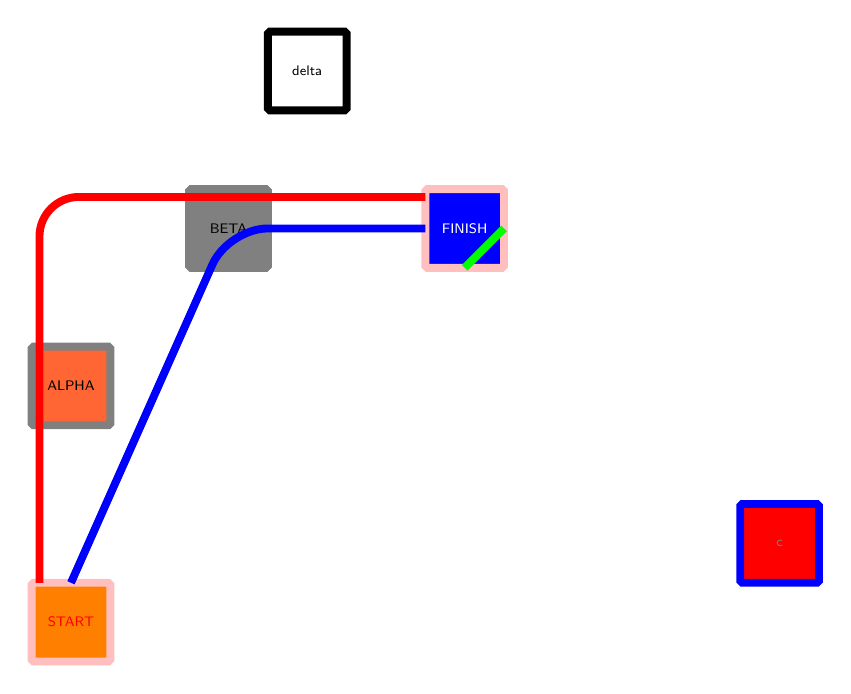
\begin{tikzpicture}
    [>={Stealth[scale=1.0]},  % Uniform arrow style
    ]
    
\node[shape=rectangle, fill=orange, draw=pink, minimum width=1cm, minimum height=1cm, rounded corners=0.025cm, line width=0.1cm, text opacity=1, font=\tiny] (node_a) at (2,2) {\textcolor{red}{START}};
\node[shape=rectangle, fill=blue, draw=pink, minimum width=1cm, minimum height=1cm, rounded corners=0.025cm, line width=0.1cm, text opacity=1, font=\tiny] (node_b) at (7,7) {\textcolor{white}{FINISH}};
\node[shape=rectangle, fill=red, draw=blue, minimum width=1cm, minimum height=1cm, rounded corners=0.025cm, line width=0.1cm, text opacity=1, font=\tiny] (node_c) at (11,3) {\textcolor{gray}{c}};
\node[shape=rectangle, fill=colorff6633, draw=gray, minimum width=1cm, minimum height=1cm, rounded corners=0.025cm, line width=0.1cm, text opacity=1, font=\tiny] (node_alpha) at (2,5) {ALPHA};
\node[shape=rectangle, fill=gray, draw=gray, minimum width=1cm, minimum height=1cm, rounded corners=0.025cm, line width=0.1cm, text opacity=1, font=\tiny] (node_beta) at (4,7) {BETA};
\node[shape=rectangle, fill=white, draw=black, minimum width=1cm, minimum height=1cm, rounded corners=0.025cm, line width=0.1cm, text opacity=1, font=\tiny] (node_delta) at (5,9) {delta};
\draw[draw=blue,line width=0.1cm,rounded corners=0.5cm] (2,2.5) -- (4,7) -- (6.5,7);
\draw[draw=red,line width=0.1cm,rounded corners=0.5cm] (1.6,2.5) -- (1.6,7.4) -- (6.5,7.4);
\draw[draw=green,line width=0.1cm,rounded corners=0.5cm] (7.5,7) -- (7,6.5);

\end{tikzpicture}
\end{document}
